\documentclass[a4paper]{exam}

\usepackage{amsmath,amssymb, amsthm}
\usepackage{geometry}
\usepackage{graphicx}
\usepackage{hyperref}
\usepackage{titling}
\usepackage{tikz}
\usepackage{tikz-qtree}

\graphicspath{{images/}}


\newtheorem{definition}{Definition}
\newtheorem{theorem}{Theorem}
\newtheorem{corollary}{Corollary}
\newtheorem{axiom}{Axiom}
\newcommand{\lcm}{\emph{lcm}}

% Header and footer.
\pagestyle{headandfoot}
\runningheadrule
\runningfootrule
\runningheader{CS/MATH 113, SPRING 2025}{Pset 08: Induction}{\theauthor}
\runningfooter{}{Page \thepage\ of \numpages}{}
\firstpageheader{}{}{}

% \printanswers %Uncomment this line

\title{Problem Set 08: Induction}
\author{Blingblong} % <=== replace with your student ID, e.g. xy012345
\date{CS/MATH 113 Discrete Mathematics\\Habib University\\Spring 2025}


\qformat{{\large\bf \thequestion. \thequestiontitle}\hfill}
\boxedpoints


\begin{document}
\maketitle      


\section*{Problems}
\begin{questions}
  \titledquestion{The sword of independence} Legend has it that underneath Teen Talwar Clifton lies the secret sword of Pakistan. Whose wielder is destined to rule Tokyo. After finding a map at the back of declaration of independence, you and your Nicholas Cage are on a quest to find this legendary sword. But the Sage of Hyderabad has told you the only way to get to the sword is to solve the puzzle left by Quaid e Azam himself. You are given $n$ disks of various sizes that would be stacked on the first sword in Teen Talwar (Unity) in descending order of size (the smallest disk on top and the largest disk on bottom). Your task is to move this stack of disks from the first sword to the last sword (Discipline). But heres the catch, you can only move one disk at a time. Furthermore you can never put a larger disk on top of a smaller disk or the entire structure will collapse. The real challenge that Quaid e Azam left is that you need to use the minimum number of moves to move the disks from the first sword to the last one. For any $n\in \mathbb{Z}^+$, let $f(n)$ be the minimum number of moves needed to move the disks from first sword to the last sword. Find an expression for $f(n)$ in terms of $n$ and prove that your expression is correct. In other words prove that the expression you propose indeed gives us $f(n)$.

\begin{figure}[h!]
  \centerline{\includegraphics[scale = 0.3]{Adnan_Asim's_Karachi_City._3_Talwar_(_Swords_)_Clifton,_Karachi.jpg}}
  \caption{Teen Talwar, Clifton, Karachi.
  Note: The image is taken from \href{https://simple.wikipedia.org/wiki/Teen_Talwar}{\url{https://simple.wikipedia.org/wiki/Teen_Talwar}}}
\end{figure}

  \begin{solution}
    % Enter solution here.
  \end{solution}

  \titledquestion{Return of the WuShrek} Consider the the WuShrek board below (on left), and the SonicChikaFreddy tiles next to it (below to the right). A SonicChikaFreddy tile would cover three squares of a WuShrek board. Imagine you have an arbitrarily large supply of SonicChikaFreddy tiles. For some $n \in \mathbb{Z}^+$, given a $2^n \times 2^n$ WuShrek board (the WuShrek board given below is $2^3\times 2^3$), show that its always possible to tile a $2^n \times 2^n$ WuShrek board with any one square removed by using SonicChikaFreddy tiles.
  \begin{center}
      \includegraphics[scale = 0.25]{WuShrekSonicChikaFreddy.png}
  \end{center}
  \begin{solution}
    % Enter solution here.
  \end{solution}
  
  \titledquestion{Pyramid Scheme}
    Suppose we have circular coins, a lot of them and all of the same dimension, and we were to make a hexagonal pyramid out of them as follows. The top layer has $1$ coin. The second layer has $7$ coins arranged in a hexagon with side length of two coins (see picture below). The third layer has $19$ coins in the same hexagonal pattern but with side length of three coins, and so on.

    Prove that a pyramid created in this manner and constituting $n$ layers requires in total $n^3$ coins.
  \begin{figure}[h!]
    \centerline{\includegraphics[scale = 0.5]{layer1}}
    \caption{Top layer as seen from above.}
    \label{layer1}
  \end{figure}
  \begin{figure}[h!]
    \centerline{\includegraphics[scale = 0.5]{layer2.png}}
    \caption{The second layer as seen from above. Note that this layer has $7$ coins and forms a hexagon with side length of two coins.}
    \label{layer2}
  \end{figure}
  \newpage
  \begin{figure}[h!]
    \centerline{\includegraphics[scale = 0.5]{layer3.png}}
    \caption{The third layer with $19$ coins forming a hexagon with side length of three coins.}
    \label{layer3}
  \end{figure}

  Note: All figures in this problem are taken from \href{https://www.geogebra.org/m/cnqdjcph}{beckykwarren's geogebra page}.

  \begin{solution}
    % Enter your solution here.
  \end{solution}

  \titledquestion{All horses are of same color} Consider the following proof that shows that all horses are of same color:
  \begin{theorem}
      In any finite set of horses all horses are always of the same color.
  \end{theorem}
  \begin{proof}
      Let $H$ be a finite set of horses, we will prove by induction (induct on $|H|$) that all horses in $H$ are of same color. 
      
      \textbf{Base case:} $|H| = 1$, if $|H| = 1$ then there is one horse in the set and so trivially all the horses in the set have same color. 

      \textbf{Induction hypothesis:} Suppose for $|H| = k$ all horses in $H$ are of same color.

      \textbf{Induction step:} Suppose $|H| = k+1$, lets take out a horse $x$ from $H$ the set $|H - \{x\}| = k$, by induction hypothesis we know that all horses in $H - \{x\}$ are of same color and as $\{x\}$ is a set of one horse all horses in $\{x\}$ are of same color. Now we consider the set $H \setminus \{y\}$ for $y \neq x$ then by the induction hypothesis again all horses in $H - \{y\}$ are of the same color and now as $x \in H - \{y\}$, $x$ has the same color as all the horses in $H \setminus \{y\}$, and therefore $x$ has the same color as all the horses in $H \setminus \{x\}$. And so all the horses in $H$ have the same color.

      So by the principles of Mathematical induction we have that in any finite set of horses, all horses have the same color.
  \end{proof}

  Is th above proof correct? If not explain what is the error in the above reasoning.
  \begin{solution}
    % Enter solution here.
  \end{solution}

  \titledquestion{Gamer smell} Your friend Goku who is a programer, gamer and likes anime has successfully gone three months without showering. Due to this you forbade Goku from coming to the anime convention unless he showers. ``But showering is for losers'' said Goku as he plans on sneaking into the convention anyways. You plan on carrying a bucket of water and soap to throw over Goku's head the minute you find him. But as everyone in the convention is in cosplay it is difficult to spot the Goku visually. Instead you are relying on the fact that Goku smells like a rotten fish. Your own sense of smell is overpowered by all the other weird convention smells. So you are going to question the other cosplayers at the convention who possess a keener sense of smell. Due to differences in olfactory systems among the cosplayers, the set of people that smell like rotten fish varies for each person. Goku however is special as he hasn't showered for three months he smells like rotten fish to everyone and also does not perceive the rotten fish smell from anyone else. To keep your interaction with the weebs to minimum, the only question you will ask a cosplayer is whether someone smells like the rotten fish to them.
  
  Use mathematical induction to show that if there are $n$ cosplayers at the convention, then you can find Goku, if he is attending, with a total of at most $3(n - 1)$ questions.
  
  \begin{figure}[h!]
    \centering
    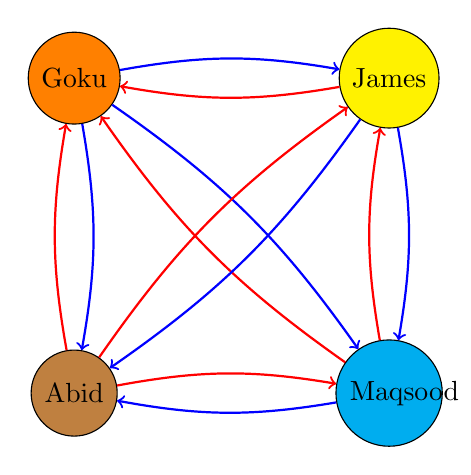
\begin{tikzpicture}
        \node [style={circle,draw, fill=brown}] (A) at (0,0) {Abid};
        \node [style={circle,draw,fill = orange}] (B) at (0,4) {Goku};
        \node [style={circle,draw, fill = cyan,text width=10mm}] (C) at (4,0) {Maqsood};
        \node [style={circle,draw, fill = yellow}] (D) at (4,4) {James};
        
        \draw[->, thick, red] (A) edge [bend left=10] (B) ;
        \draw[->, thick, red] (C) edge [bend left=10] (B) ;
        \draw[->, thick, red] (D) edge [bend left=10](B) ;
        \draw[->, thick, blue] (B) edge[bend left=10] (A) ;
        \draw[->, thick, blue] (B) edge[bend left=10] (C) ;
        \draw[->, thick, blue] (B) edge[bend left=10] (D) ;

        \draw[->, thick, red] (A) edge [bend left=10] (C) ;
        \draw[->, thick, red] (A) edge [bend left=10] (D) ;

        \draw[->, thick, blue] (D) edge[bend left=10] (A) ;
        \draw[->, thick, blue] (D) edge[bend left=10] (C) ;

        \draw[->, thick, red] (C) edge[bend left=10] (D) ;
        \draw[->, thick, blue] (C) edge[bend left=10] (A) ;

    \end{tikzpicture}
   
    
    \caption{An example of four cosplayers smelling each other, the blue arrow from cosplayer $X$ to cosplayer $Y$ represents that $Y$ doesn't smells like rotten fish to $X$ and a red arrow from cosplayer $X$ to cosplayer $Y$ represents that $Y$ smells like rotten fish to $X$. Here we can see that Goku is the only person that smells like rotten fish to everyone nd no one smells like rotten fish to Goku.}
\end{figure}

  \begin{solution}
    % Enter solution here.
  \end{solution}
  

  
  
  \titledquestion{Bonus Problem} The following problem is optional to attempt: 
  
  Show that the principle of mathematical induction is a valid proof technique. 

  (Hint: look up the well ordering principles, how does it helps us to show that mathematical induction is a valid proof technique. You can take well ordering principle as an axiom here.)
  \begin{solution}
    % Enter solution here.
  \end{solution}
  
\end{questions}


\end{document}

%%% Local Variables:
%%% mode: latex
%%% TeX-master: t
%%% End:
